% last updated in April 2002 by Antje Endemann
% Based on CVPR 07 and LNCS, with modifications by DAF, AZ and elle, 2008 and AA, 2010, and CC, 2011

\documentclass[runningheads]{llncs}
\usepackage{graphicx}
\usepackage{amsmath,amssymb} % define this before the line numbering.
\usepackage{ruler}
\usepackage{color}
\usepackage{epsfig}
\usepackage{booktabs}
\usepackage{verbatim}
\usepackage{array}
\usepackage{xspace}

\usepackage[width=122mm,left=12mm,paperwidth=146mm,height=193mm,top=12mm,paperheight=217mm]{geometry}

\usepackage{alexfmacros}
\begin{document}

% \renewcommand\thelinenumber{\color[rgb]{0.2,0.5,0.8}\normalfont\sffamily\scriptsize\arabic{linenumber}\color[rgb]{0,0,0}}
% \renewcommand\makeLineNumber {\hss\thelinenumber\ \hspace{6mm} \rlap{\hskip\textwidth\ \hspace{6.5mm}\thelinenumber}}
% \linenumbers

\pagestyle{headings}
\mainmatter
\def\ECCV12SubNumber{***}  % Insert your submission number here

%\title{Structured Prediction for Manhattan Scene Understanding}
%\title{Predicting structured geometry from single and multiple views}
% Replace with your title

\titlerunning{ECCV-12 submission ID \ECCV12SubNumber}

\authorrunning{ECCV-12 submission ID \ECCV12SubNumber}

\author{Anonymous ECCV submission}
\institute{Paper ID \ECCV12SubNumber}

\maketitle

\begin{abstract}
  We develop a structured prediction approach to reconstructing 3D
  polygonal models from single and multiple images of a
  scene. Building on recent advances in single view reconstruction we
  adopt the indoor Manhattan hypothesis class --- one of the most
  complicated output spaces (in terms of internal constraints) yet
  considered within a structured prediction framework. Our approach
  can learn in both the single-- and multiple--view contexts. We
  show that the chosen hypothesis class permits optimizing a variety
  of high--level loss functions, such as the relative depth error. Our
  results out--perform the state--of--the--art, including an
  improvement of more than $50\%$ on one metric.
\end{abstract}

\section{Introduction}
\label{sec:introduction}

Reconstruction 3D models from images is a central problem in computer
vision. There is a deep literature concerning reconstruction from
multiple views of a scene, with particular focus on the geometry of
multiple cameras. More recently the recovery of 3D information from a
single image has received attention \cite{Hoiem05,Saxena09}. In this
context the geometric constraints leveraged by multiple--view
reconstructors are unavailable, so inference must rely on photometric
cues. To capture the complex, high--dimensional patterns involved in
this challenging inference task, practitioners have leveraged a range
of machine learning techniques.

Within single--view reconstruction, few authors have cast learning as
a single optimisation with respect to a clearly defined loss function
\cite{Hoiem05,Saxena09,Lee09,Flint11}, while most approaches to
multiple--view reconstruction do not consider learning from training
data at all. In contrast, this paper casts reconstruction
fundamentally as a learning problem, with the goal being to learn a
prediction function $\Predictor$ mapping observed features to 3D
reconstructions.

Building on recent advances in single--view reconstruction we adopt as
our hypothesis class the set of indoor Manhattan models
\cite{Lee09,Flint10eccv,Flint11}, under which scenes are approximated
by a floor and ceiling plane together with a sequence of vertical
walls. This representation brings a variety of attractive features
such as a simple parametrisation, efficient and exact inference,
decomposability of loss functions, and a balance between
expressiveness and robustness.

For learning we employ the tools of structured prediction, in
particular the structural SVM \cite{Tsochantaridis04}. The use of
these tools is part part of a long trend towards statistically
rigorous, well--understood convex optimization techniques in computer
vision. Recent successfully applications include detection
\cite{blaschko2008learning}, segmentation \cite{taskar2004max}, and
scene classification \cite{Yang2010}. In the domain of reconstruction,
structured prediction ideas have been applied to several simple models
classes such as stereo disparities \cite{li2008learning} and cuboids
\cite{Hedau09}.

The application of structured prediction to the indoor Manhattan class
of models constitutes one of the most complex output spaces yet
considered within this framework. The indoor Manhattan model enforces
hard geometric constraints that lack simple expressions in terms of
image coordinates. These constraints are context--dependent, being
tied to quantities such as camera rotation and the location of
vanishing points. We have learnt several valuable lessons of general
relevance from this complex prediction task, to which we dedicate the
final section of this paper.

The contributions of this paper are thus (i) a unified learning
framework for single-- and multiple--view reconstruction, utilising
the indoor Manhattan model and the tools of structured prediction;
(ii) the reduction of two image--level loss functions to a form
amenable to efficient optimization; (iii) an efficient separation
procedure for identify the ``most--violated constraint'' during
learning, (iv) an empirical demonstration of structured prediction in
perhaps the most complex output space yet considered within this
framework; and (v) a series of practical observations concerning the
application of structured prediction techniques.

In the remainder of this paper we present background material
(\secref{background}), followed by the indoor Manhattan model itself
(\secref{model}), and our learning framework (\secref{learning}). We
then present results for multiple--view reconstruction
(\secref{mv-results}) followed by single--view reconstruction
(\secref{sv-results}), then we close with practical lessons learnt
(\secref{discussion}) and concluding remarks (\secref{conclusion}).

\section{Background}
\label{sec:background}

This paper touches on several major research areas (multiple--view
reconstruction, single--view reconstruction, and structured
prediction), so here we present only key contributions and those
results of particular relevance to our own work.

Multiple view reconstruction has a long history in the literature,
beginning at least as early as the seminal work of Marr \etal
\cite{Marr1976}. Low--level approaches estimate the depth of each
pixel by solving for stereo disparity (for a survey see
\cite{Scharstein2002}), while high--level approaches attempt to
recover polyhedral models of various kinds
\cite{Baillard1999,Liebowitz1999}. The present work follows the spirit
of the latter approach.

Coughlan and Yuille \cite{Coughlan99} first introduced the Manhattan
world assumption, in which reconstructed surfaces are restricted to three
mutually--orthogonal orientations. Furukawa \etal \cite{Furukawa09}
applied this idea within a multiple view stereo context. Lee \etal
\cite{Lee09} proposed the indoor Manhattan assumption, which places
further restrictions on reconstructed models.

Single--view reconstruction from line drawings also has a long history
in the literature (\cite{Huffman71}, for example). Reconstructing
single real--world images was re--introduced to the community by Hoiem
\etal \cite{Hoiem05}, who employed decision trees to classify image
segments into orientation classes in a multiple segmentation
approach. Saxena \etal \cite{Saxena09} employed energy minimisation to
recover pixel--wise depths. Barinova \etal \cite{Barinova08}
reconstructed piece--wise planar outdoor scenes using an EM
algorithm. Hedau \etal \cite{Hedau09} modelled indoor scenes as the
interior of a cuboid, and cast learning within a structured prediction
framework. We also use structured prediction, though our hypothesis
class is far more expressive.

Lee \etal \cite{Lee09} were the first to reconstruct indoor Manhattan
scenes. They devised a combinatorial search over line segments using a
branch--and--bound algorithm. Flint \etal
\cite{Flint10eccv} refined this to an exact dynamic
programming solution, and in later work \cite{Flint11} extended the
indoor Manhattan assumption to the multiple view domain. The authors
of \cite{Flint11} did describe a learning algorithm based on
bootstrapping, though its statistical consistency was given little
attention. The present work relies extensively on this thread of
research, though in contrast to past work our focus is entirely on
learning in a statistically rigorous framework. We provide comparisons
with these approaches.

Extending binary and multi--label classification to general output
spaces is a major research programme within the machine learning
community; an excellent introduction is given by Bakir \etal
\cite{Bakir07}. Our approach employs the structured support vector
machine, first proposed by Tsochantaridis \etal
\cite{Tsochantaridis04} and improved upon by Joachims \etal
\cite{Joachims2009}.

\section{Model}
\label{sec:model}

In this section we describe three components of the model that we are
trying to learn (and, at test time, infer): a hypothesis class, a
feature space, and a loss function. In our setup these are,
respectively, the class of indoor Manhattan models, a log--linear
Bayesian likelihood, and either the relative depth error or a
labelling error (we describe both).

\subsection{Hypothesis Class}

This paper is concerned with the hypothesis class consisting of indoor
Manhattan reconstructions, which are 3D polygonal models characterized
by infinite floor and ceiling planes with vertical walls extending
between them (as originally proposed by Lee \etal
\cite{Lee09}). Indoor Manhattan environments are a sub--class of
general Manhattan environments; examples are shown in figure
\figref{indoor-manhattan}. This is an attractive hypothesis class
because
\begin{enumerate}
\item{it captures many regularities within man--made environments;}
\item{the geometric primitives (floor/wall/ceiling) are immediately
  useful for semantic--level scene understanding;}
\item{it is expressive enough to represent approximately or exactly
  a surprisingly wide variety of environments;}
\item{there is a simple and convenient parametrisation;}
\item{an efficient inference algorithm exists \cite{Flint10eccv}.}
\end{enumerate}

\begin{figure}[tb]
  \centering
  \subfloat[]{
    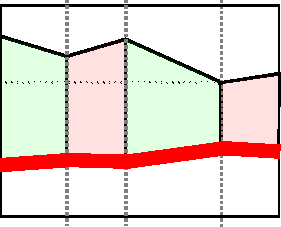
\includegraphics[width=0.3\textwidth]{figures/example-model1}
  }
  \subfloat[]{
    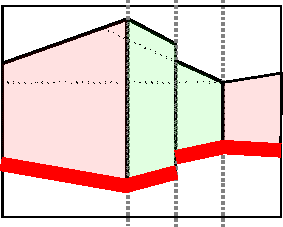
\includegraphics[width=0.3\textwidth]{figures/example-model2}
  }
  \subfloat[]{
    \includegraphics[width=0.3\textwidth]{figures/example-floorplan}
  }
  \caption{(a-b) Examples of indoor Manhattan environments. The red
    line illustrates the seam representation. (c)
    An indoor Manhattan environment viewed from above.}
  \label{fig:indoor-manhattan}
\end{figure}

An indoor Manhattan model is much like an archicetural floor--plan,
and can be specified as a set of 2D line segments representing walls
together with the position of the floor and ceiling plane
(\figref{indoor-manhattan}). In this paper we adopt an image--domain
parametrisation due to its convenience for inference and
learning. Following Flint \etal \cite{Flint11} we represent hypotheses
as a path running from the left edge to the right edge of the image,
which we will refer to as a \textit{seam}. A seam $\Seam$ consists of
a sequence of pairs of scalars,
\begin{equation}
  \Seam = \{\seam_i,\Label_i\}_{i=1}^{\Width}
\end{equation}
where $\seam_i$ is the $y$--coordinate at which the path intersects
image column $i$, $\Label_i$ is the orientation of the wall in that
column, and $\Width$ is the image width. Remarkably, this simple
parametrisation specifies a unique metric 3D model up to scale
\cite{Flint11}.

While we do not here have space for a full discussion of the geometry
of indoor Manhattan models, there are two properties of the seam
representation that will be relevant in the following
sections. Firstly, images of indoor Manhattan environments can be
rectified so that vertical lines in the world project to vertical
lines in the image \cite{Flint10eccv}. Secondly, the mapping from seam
to 3D reconstruction decomposes in the following manner. We said
earlier that a seam $\Seam$ specifies a unique 3D reconstruction. Let
$\Orient(x,y;\Seam)$ be the orientation of the 3D
surface projecting to pixel $(x,y)$. Flint \etal \cite{Flint10eccv}
showed that $\Orient$ is functionally dependant \textit{only} on the
pair $(\seam_x,\Label_x)$ for column $x$. That is, we may write
\begin{equation}
  \label{eq:orient-indep}
  \Orient(x,y;\Seam) = \tilde{\Orient}(x,y;\seam_x,\Label_x) ~.
\end{equation}
Similarly, letting $\Depth(x,y,;\Seam)$ be the distance from the
camera to the surface projecting to $(x,y)$ we may write
\begin{equation}
  \label{eq:depth-indep}
  \Depth(x,y;\Seam) = \tilde{\Depth}(x,y;\seam_x,\Label_x) ~.
\end{equation}

\subsection{Feature Space}

We adopt the probabilistic model formulated by Flint \etal
\cite{Flint11}, which relates indoor Manhattan reconstructions to
single--view image features, multiple--view photo--consistency terms,
and a reconstructed point cloud. From our perspective these are simply
features and any subset may be omitted if inappropriate for a given
application. Under this model the prior on reconstructions is
\begin{equation}
  \log P(\Seam) = - \vect{n} \cdot \Penalties + O(1)
  \label{eq:prior}
\end{equation}
where $\vect{n}$ is a vector containing the number of walls in $\Seam$
of various categories (concave, convex, occluding) and $\Penalties$ is
a hyper--parameter. We may interpret \eqnref{prior} as,
roughly, that reconstructions with more walls are less likely.

Flint \etal \cite{Flint11} showed that for a variety of features
$\Feature$ (including single--view and multiple--view) there are
reasonable choices of likelihood that can be written
\begin{equation}
  \log P(\Feature ~|~ \Seam) = \sum_{x=1}^\Width 
  \PixelPayoff_{\Feature}(x,\seam_x)
  \label{eq:likelihood}
\end{equation}
where $\PixelPayoff_{\Feature}$ is a real matrix computed
deterministically from $\Feature$ and $\PixelPayoff_{\Feature}(i,j)$
is the element at row $i$, column $j$. It is easy to show that for each
sensor model described in \cite{Flint11} the log--likelihood is linear
in the hyper--parameters $\LikelihoodHypers$, \ie
\begin{equation}
  \log P(\Feature ~|~ \Seam) = 
  \sum_{x=1}^\Width
  \LikelihoodHypers_{\Feature} 
  \cdot
  \PixelFtr_{\Feature}(x,\seam_x) ~.
\end{equation}
Assuming conditional independence between features, the posterior is
\begin{eqnarray}
    P(\Seam ~|~ \Features)
  &\propto&
    P(\Seam) \prod_{i=1}^n P(\Feature_i ~|~ \Seam)\\
    \log P(\Seam ~|~ \Features)
  &=&
    - \vect{n} \cdot \Penalties
    + \sum_{i=1}^n \sum_{x=1}^\Width 
    \LikelihoodHypers_i \cdot \PixelFtr_i(x,\seam_x)
    + O(1) ~.
  \label{eq:log-posterior}
\end{eqnarray}

So far, this model closely follows that described in \cite{Flint11};
our contribution is to place this model into a statistically rigorous
learning framework. To do this we need to rewrite the above in terms
of a joint feature function $\JointFtr(\Features,\Seam)$ and a
parameter vector $\Model$. The decomposability of indoor Manhattan
models into payoff matrices permits precisely such a
formulation. Defining
\begin{align}
  \JointFtr(\Features,\Seam) =
  \begin{bmatrix}
    -\vect{n} \\
    \sum_{x=1}^\Width \PixelFtr_1(x,\seam_x) \\
    \vdots \\
    \sum_{x=1}^\Width \PixelFtr_n(x,\seam_x)
  \end{bmatrix}
  & \quad &
  \Model =
  \begin{bmatrix}
    \Penalties \\
    \LikelihoodHypers_1 \\
    \vdots \\
    \LikelihoodHypers_n
  \end{bmatrix}
  \label{eq:joint-ftr-def}
\end{align}
we see that \eqnref{log-posterior} can be written as
\begin{equation}
  \log P(\Seam ~|~ \Features)
  =
  \bigl\langle \Model ~,~ \JointFtr(\Features,\Seam) \bigr\rangle +
  O(1)
  \label{eq:log-linear-posterior}
\end{equation}
where we have adopted Hilbert space notation with
$\langle\cdot,\cdot\rangle$ denoting an inner product. Since $\Model$
contains all free parameters in the model, the goal of learning will
be to optimise $\Model$ with respect to a training set
$\{(\Features_i,\Seam_i)\}$. 

\subsubsection{Features}

The precise make--up of the feature space depends on the available
sensor modalities. We define separate feature spaces for the single--
and multiple--view contexts; these are summarized in
\figref{featurespace}.

\begin{figure}[tb]
  \centering
  \begin{tabular}{@{}lllll@{}}
    \toprule
    Feature & Dimensionality & Multi--view? & Single--view? & Reference \\
    \midrule
    Stereo photo--consistency & 4 & yes & no & Flint \etal \cite{Flint11}\\
    Point cloud & 2 & yes & no & Flint \etal \cite{Flint11}\\
    Line sweeps & 1 & yes & yes & Lee \etal \cite{Lee09}\\
    RGB+HSV & 6 & no & yes & \\
    Gabor responses\footnotemark & 12 & no & yes & \\
    \bottomrule
  \end{tabular}
  \caption{The composition of our single-- and multiple--view feature
    space. We omit color and Gabor features from the multiple--view
    feature space for training efficiency.}
  \label{fig:featurespace}
\end{figure}


\subsection{Loss Functions}

\footnotetext{4 orientations, 3 scales}

Next we define a loss function $\Delta(\Seam,\EstSeam)$ measuring the
cost of predicting some reconstruction $\EstSeam$ when in fact the
true reconstruction is $\Seam$. In the context of learning one often
faces a trade--off between choosing a loss that leads to tractable
optimization, and choosing a loss that measures the quantity that one
``really'' cares about. For example, Hoiem \etal \cite{Hoiem05} learn
a per--segment orientation classifier, then pass this as input to a
separate 3D reconstruction system \cite{Hoiem2005}. However, what one
``really'' cares about is some loss defined on the output of the
entire system rather than the output of individual components, since
some segment--level mistakes are insignificant to the overall
reconstruction quality, while others are catastrophic. This is not a
criticism of the authors' choice, but an illustration of the
trade--off faced when choosing a loss. In this paper we show how to
learn efficiently with respect to a loss defined on the final
reconstruction.

The relative depth error has been the gold standard within the
reconstruction community for more than a decade \cite{Hartley04}, and
measures the average deviation between reconstructed and ground truth
depths. In our notation,
\begin{equation}
  \label{eq:depth-loss}
  \DepthLoss(\Seam,\EstSeam)
  =
  \frac{1}{N}
  \sum_{\Pixel}
  \frac
      {\abs{\Depth(\Pixel;\EstSeam) - \Depth(\Pixel;\Seam)}}
      {\Depth(\Pixel;\Seam)} ~,
\end{equation}
where $N$ is the number of pixels. Another reasonable choice is the
labelling error, used widely within the semantic segmentation
literature,
\begin{equation}
  \label{eq:label-loss}
  \LblLoss(\EstSeam,\Seam)
  =
  \frac{1}{N}
  \sum_{\Pixel}
  \bigl[~\Orient(\Pixel;\EstSeam) \neq \Orient(\Pixel;\Seam)~\bigr] ~,
\end{equation}
where $[p]$ is 1 if $p$ is true and 0 otherwise. An attractive
characteristic of the indoor Manhattan class is that \textit{both of
  these losses can be optimized exactly}. The algorithmic details are
left to \sectref{learning}; the key result we establish here is that
$\DepthLoss$ and $\LblLoss$ can be written in a form resembling the
payoff formulation \eqnref{likelihood} for the feature likelihoods.

First we invoke the independence established in \eqnref{depth-indep}:
\begin{equation}
  \DepthLoss(\EstSeam,\Seam)
  =
  \frac{1}{N}
  \sum_{x=1}^{\Width}
  \sum_{y=1}^{\Height}
  \frac
      {\abs{\tilde{\Depth}(x,y;\hat{\seam}_x) - \Depth(x,y;\Seam)}}
      {\Depth(x,y;\Seam)} ~.
\end{equation}
Defining a real matrix $\LossMat_{\Seam}$,
\begin{equation}
  \LossMat_{\Seam}(x,j) =
  \sum_{y=1}^H
  \frac
      {\abs{\tilde{\Depth}(x,y;j) - \Depth(x,y;\Seam)}}
      {\Depth(x,y;\Seam)} ~,
\end{equation}
we see that we can write $\DepthLoss$ in the form
\begin{equation}
  \DepthLoss(\EstSeam,\Seam)
  =
  \frac{1}{N}
  \sum_{x=1}^{\Width} \LossMat_{\Seam}(x,\hat{\seam}_x) ~.
  \label{eq:depth-loss-matrix}
\end{equation}
There is a similar form for $\LblLoss$, which we omit here due to
space constraints.

\subsubsection{Choosing a Loss Function}

Neither of the above losses is unequivocally the ``correct'' loss; the
choice will depend on the application. One might expect a strong
correlation between the losses, and indeed one can show analytically
that
\begin{equation}
  \DepthLoss(\EstSeam,\Seam) = 0
  \iff
  \LblLoss(\EstSeam,\Seam) = 0 ~.
\end{equation}
However, in our experiments we found only a weak correlation between
these losses away from the origin. For example, the scatter plot shown
in figure \figref{comparative-scatter} shows a significant number of
outliers that score very well on $\DepthLoss$ but poorly on
$\LblLoss$, and vice versa.

\section{Learning}
\label{sec:learning}

We turn now to the problem of learning within the model described
above. Our learning task is to identify a prediction function
$\Predictor$ mapping observed features $\Features$ to reconstructions
$\Seam$. We seek the loss minimizer
\begin{equation}
  \OptPredictor = 
  \argmin_{\Predictor} 
  \Expected \Bigl[ 
    \Loss\bigl(\Predictor(\Features),\Seam\bigr)
    \Bigr] ~,
\end{equation}
which we approximate in the framework of empirical risk minimization as
\begin{equation}
  \OptPredictor = 
  \argmin_{\Predictor} 
  \sum_k \Loss\bigl(\Predictor(\Features_k),\Seam_k\bigr) ~,
\end{equation}
where $k$ indexes a training set. To perform this optimization we
turn to the tools of structured prediction \cite{Bakir07}, and in
particular the structured SVM \cite{Tsochantaridis04}. First we need
to define $\Predictor$. In this paper we consider predictors of the
form
\begin{equation}
  \Predictor_{\Model}(\Features) = \argmax_{\Seam} 
  \bigl\langle \Model ~,~ \JointFtr(\Features,\Seam) \bigr\rangle
  ~.
  \label{eq:predictor-class}
\end{equation}
Comparing with \eqnref{log-linear-posterior} we see that each
predictor of the form \eqnref{predictor-class} is simply implementing
MAP inference under some set of hyper--parameters $\Model$. We now
turn to the optimisation problem itself. Following the standard
approach \cite{Bakir07} we cast the learning problem as a constrained
optimisation problem,
\begin{equation}
  \begin{split}
    \min_{\Model,\xi} &
      \hspace{2mm} 
    \frac{1}{2} \|\Model\|^2 +
      C \sum_{k=1}^n \xi_k\\
    s.t. & \hspace{2mm} \forall k, \Seam \neq \Seam_k:~
      \bigl\langle\Model, \JointFtr(\Features_k,\Seam_k)\bigr\rangle -
      \bigl\langle\Model, \JointFtr(\Features_k,\Seam)\bigr\rangle
      \geq
      \Loss(\Seam,\Seam_k) - \xi_k ~.
  \end{split}
  \label{eq:svm-problem}
\end{equation}
Tsochantaridis \etal \cite{Tsochantaridis04} described an algorithm
for solving this minimisation that is now used extensively within
machine learning and computer vision. To apply this algorithm here we
must solve two inference problems:
\begin{enumerate}
  \item{\textit{Prediction.} This is the maximization described in
    \eqnref{predictor-class}.}
  \item{\textit{Separation.} The algorithm described in
    \cite{Tsochantaridis04} requires a user--supplied procedure to
    find the ``most--violated constraint'' at each iteration. That is,
    \begin{equation}
      \argmax_{\Seam}
        \bigl\langle\Model, \JointFtr(\Features_k,\Seam)\bigr\rangle
        + \Loss(\Seam,\Seam_k) ~.
        \label{eq:separation-problem}
    \end{equation}
  }
\end{enumerate}

Our solutions to both of the above build on the algorithm presented by Flint
\etal \cite{Flint10eccv,Flint11}, which is a dynamic programming
solution to problems of the form
\begin{equation}
  \argmax_{\Seam}
  \sum_x \PixelPayoff(x,\seam_x) - \sum_j \CornerPenalty(j;\Seam) ~.
  \label{eq:inference-problem}
\end{equation}

\subsection{Inference (Prediction)}

We showed in \secref{model} that \eqnref{inference-problem} can be
written in the form \eqnref{predictor-class}, so the prediction
problem is a straightforward application of \cite{Flint10eccv}. This
is as expected since, as we have already remarked,
\eqnref{predictor-class} is equivalent to MAP inference on indoor
Manhattan reconstructions, which was precisely the subject
of \cite{Flint10eccv}.

\subsection{Loss--Augmented Inference (Separation)}

It turns out that the separation problem can also be solved using the
dynamic programming algorithm mentioned above, as the following
proposition shows.

\begin{proposition}
  Let $(\Features_k,\Seam_k)$ be a training instance with payoff
  matrices $\{\PixelPayoff_i\}$ as defined in \eqnref{likelihood}.
  Let
  \begin{equation}
    \AugPayoff = \LossMat_{\Seam_k} + \sum_i \PixelPayoff_i ~.
    \label{eq:aug-payoff}
  \end{equation}
  Then the solution to \eqnref{inference-problem} with
  $\PixelPayoff=\AugPayoff$ is identical to the solution to
  \eqnref{separation-problem}.
\end{proposition}
\begin{proof}
  Direct equivalence of the expressions to be maximized. First
  substitute \eqnref{log-linear-posterior} and
  \eqnref{depth-loss-matrix} into \eqnref{inference-problem}:
  \begin{equation}
    \log P(\Seam ~|~ \Features) +
    \sum_{x=1}^{\Width} \LossMat_{\Seam_k}(x,\seam_x) ~
  \end{equation}
  Further substituting \eqnref{likelihood} and defining
  $\CornerPenalty$ as in \cite{Flint11} gives
  \begin{equation}
    \sum_i \sum_{x=1}^{\Width} \PixelPayoff_i(x,\seam_x) - 
    \sum_j \CornerPenalty(j;\Seam) +
    \sum_{x=1}^{\Width} \LossMat_{\Seam_k}(x,\seam_x) ~.
  \end{equation}
  Finally we see that substituting \eqnref{aug-payoff} gives
  \begin{equation}
    \sum_{x=1}^{\Width} \AugPayoff(x,\seam_x) - 
    \sum_j \CornerPenalty(j;\Seam)
  \end{equation}  
\end{proof}

\section{Multiple View Results}
\label{sec:mv-results}

We evaluated our approach on the data--set proposed in \cite{Flint11},
which consists of 18 sequences of six environments averaging 59
seconds in duration. We sampled key--frames at regular intervals. Each
``instance'' in our training and hold--out sets consists of one base
frame together with four auxiliary frames.

We compared with the bootstrapping approach described in
\cite{Flint11}. Our metrics differ from theirs in two ways. Firstly,
they compute relative depth error using the maximum of the ground
truth and estimated depths in the denominator, whereas we always use
the ground truth in the denominator. These metrics are separated by at
most a monotonic transform but the latter is more convenient to
represent in our framework. Secondly, when we compute labelling error
we differentiate vertical and horizontal surfaces only, whereas they
also differentiate the two vertical orientations. The latter approach
makes a side--by--side comparison difficult because the two vertical
orientations are symmetric and their labels can always be
interchanged.

The performance of these two algorithms are summarized in
\figref{mv-performance}. Our approach significantly out--performs the
bootstrapping algorithm. Anecdotally we noticed that much of the
improvement resulted from a reduction in catastrophic failures. This
makes sense because we would expect the learning algorithm to
concentrate on reducing those mistakes that result in the largest
loss. Some example predictions are shown in \figref{results-pics};
many more are included in additional material.

\begin{figure}[tb]
  \centering
  \begin{tabular}{@{}p{20mm}p{20mm}p{20mm}p{20mm}p{20mm}@{}}
    \toprule
     & \multicolumn{2}{c}{Depth Error (\%)}
     & \multicolumn{2}{c}{Labelling Error (\%)} \\
    \midrule
    Sequence & This Paper\footnotemark[2] & Flint \etal 
             & This Paper\footnotemark[3] & Flint \etal \\
    \midrule
    \tt{ground}   & 4.9    & 66.6    & 2.9    & 10.4  \\
    \tt{foyer1}   & 6.1    & 6.6     & 3.1    & 3.1   \\
    \tt{foyer2}   & 4.3    & 5.4     & 3.7    & 4.0   \\
    \tt{corridor} & 14.6   & 52.9    & 9.5    & 19.2  \\
    \tt{mcr}      & 34.0   & 67.6    & 15.    & 16.2  \\
    \tt{kitchen}  & 16.8   & 23.6    & 5.2    & 6.1   \\
    \midrule
    Average       & \textbf{13.4} & 37.1 & \textbf{6.7} & 9.8   \\
    \bottomrule
  \end{tabular}
  \caption{Multiple--view reconstruction performance on held--out
    data, comparing with Flint \etal \cite{Flint11}. For unavoidable
    reasons we use slightly different metrics so our figures differ
    from those published in \cite{Flint11}. See main text for
    explanation.}
  \label{fig:mv-performance}
\end{figure}

\begin{figure}[tb]
  \centering
  \begin{tabular}{@{}p{20mm}p{20mm}p{20mm}p{20mm}p{20mm}@{}}
    \toprule
     & \multicolumn{2}{c}{Depth Error (\%)}
     & \multicolumn{2}{c}{Labelling Error (\%)} \\
    \midrule
    Sequence & This Paper\footnotemark[2] & Flint \etal 
             & This Paper\footnotemark[3] & Flint \etal \\
    \midrule
    \tt{ground}   & 17.3   & 24.5    & 7.8    & 12.2  \\
    \tt{foyer1}   & 25.1   & 31.0    & 15.1   & 22.2  \\
    \tt{foyer2}   & 29.1   & 30.1    & 15.9   & 18.6  \\
    \tt{corridor} & 31.7   & 33.6    & 19.3   & 24.8  \\
    \tt{mcr}      & 70.1   & 45.9    & 26.7   & 20.8  \\
    \tt{kitchen}  & 25.1   & 26.2    & 7.7    & 11.9  \\
    \midrule
    Average       & 33.1   & \textbf{31.9} & \textbf{15.4} & 18.4   \\
    \bottomrule
  \end{tabular}
  \caption{Single--view reconstruction performance on held--out data,
    comparing with Flint \etal \cite{Flint10eccv}.}
  \label{fig:sv-performance}
\end{figure}


\begin{figure}[tb]%
  \centering
  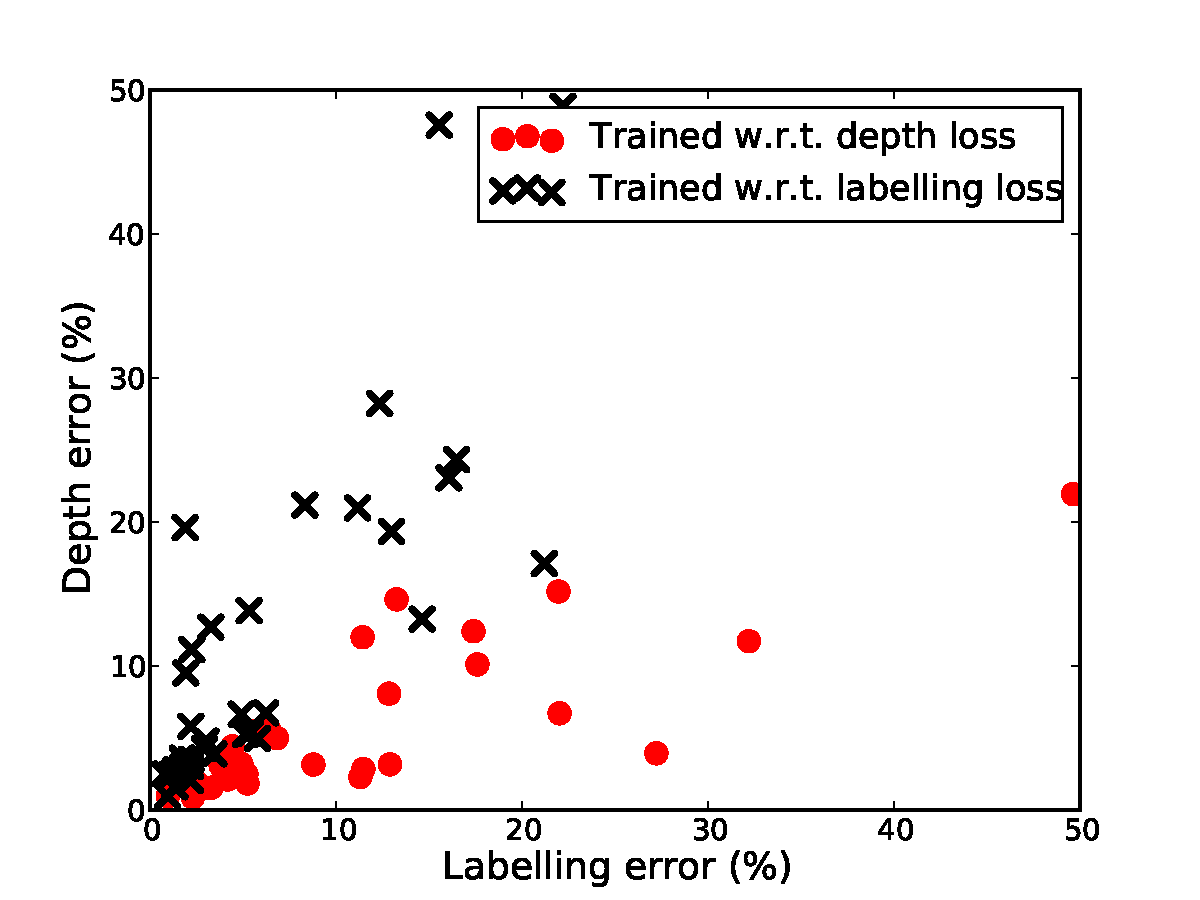
\includegraphics[width=0.6\textwidth]{figures/comparative_scatter}
  \caption{The effect of the loss function on training. We train two
    predictors, one with respect to $\DepthLoss$ and one with respect
    to $\LblLoss$, then evaluate both on all held--out instances. Each
    data point shows the error obtained by one predictor on held--out
    instance. The differing distribution of errors shows that the two
    predictors trade off errors as expected.}
  \label{fig:comparative-scatter}
\end{figure}

\begin{figure}[tb]
  \centering
  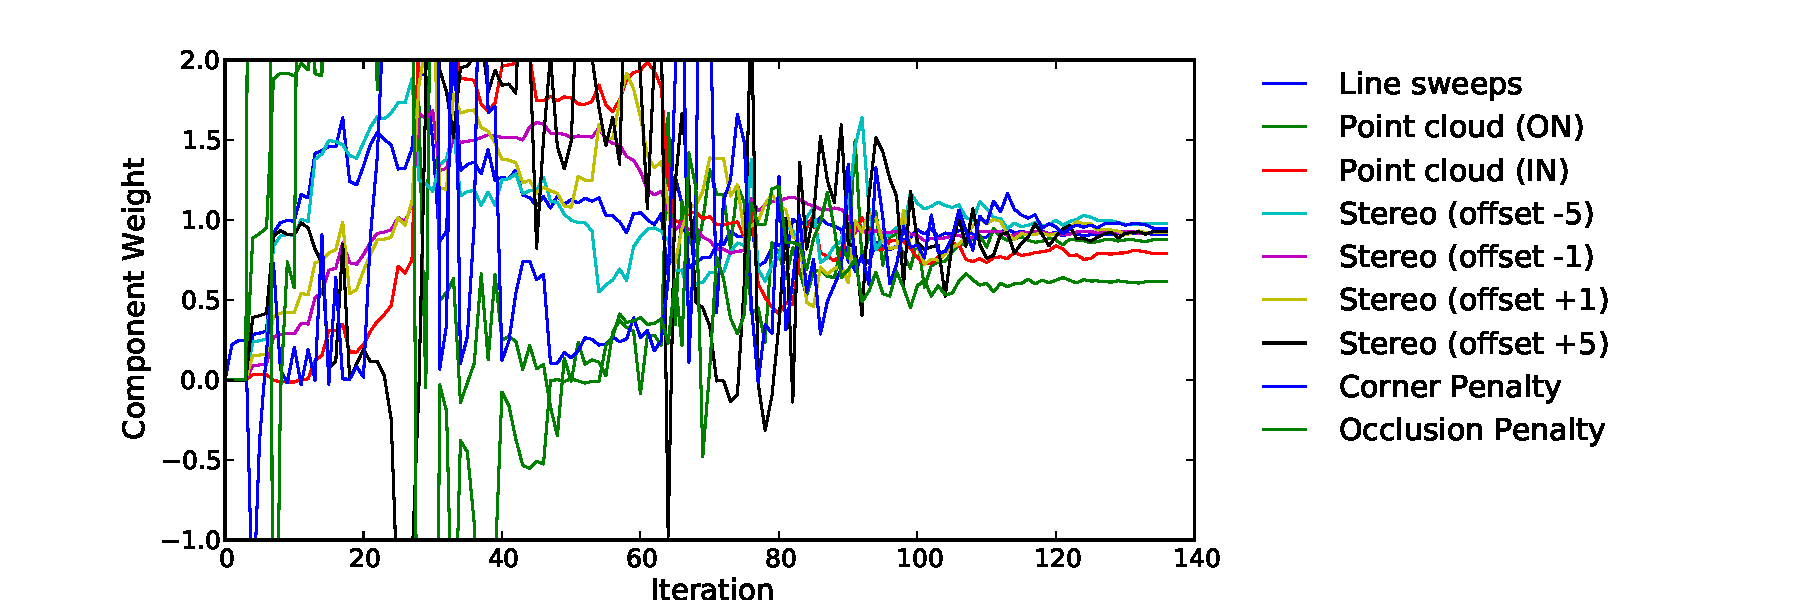
\includegraphics[width=\textwidth]{figures/psi_evolution}
  \caption{Evolution of $\Model$ during training. Each series shows
    the value of one component of $\Model$. After an
    exploration phase the model converges.}
  \label{fig:psi-evolution}
\end{figure}

\section{Single View Results}
\label{sec:sv-results}

We evaluated our system for single--view reconstruction using the same
data--set described in the previous section. We used the single--view
features summarized in \figref{featurespace}. We compared our approach
to the single--view approach of Flint \etal \cite{Flint10eccv}, which
uses the same dynamic programming algorithm that we rely upon, but
uses hand--tuned features.

Performance for each algorithm is summarized in
\figref{mv-performance}. When measured by labelling error, our
approach out--performs the hand--tuned weights, but on the depth error
metric our approach is inferior. While investigating this result we
found that our learning algorithm assigns small weights to all but the
line--sweep features, which are the same features used by
\cite{Flint10eccv}. This suggests that the hand--tuned weights are in
fact close to optimal within this feature space, though one would
expect that with additional feature engineering our learning algorithm
would be able to leverage further salient information and reduce the
error rate.

\footnotetext[2]{This column represents the predictor trained with
  respect to $\DepthLoss$.}

\footnotetext[3]{This column represents the predictor trained with
  respect to $\LblLoss$.}

\section{Discussion}
\label{sec:discussion}

The hypothesis class considered in this paper is amongst the most
complex (in terms of internal constraints on the output space) studied
within the structured prediction framework. In this section we turn to
some practical lessons learnt that may be of value to other
practitioners.

\subsubsection{Condition in the joint feature space, not the input
  feature space.}

A common pre--processing operation for statistical learning is to
transform the observed features $\Features$ to zero mean and unit
variance. However, for structured prediction tasks it is the joint
feature space $\JointFtr$ that should be conditioned:
\begin{equation}
  \label{eq:conditioning}
  \JointFtr' = \frac{\JointFtr - \mu}{\sigma^2} ~.
\end{equation}
Ideally one would sample from the joint feature space to determine the
conditioning transformation, but the distribution of inputs and
outputs is generally unknown in an empirical risk minimization
setting. Instead, we use the training set as a proxy. We compute the
empirical mean and variance of
$\{\JointFtr(\Features_k,\Seam_k)\}_{k=1}^n$ at the outset, then apply
the transformation \eqnref{conditioning} after each feature
computation.

\subsubsection{Condition the loss terms.}

For any $\eta>0$, the minimization problem \eqnref{svm-problem} is
equivalent (under the substitution $\Model'=\eta\Model$,
$\xi'=\eta\xi$) to:
\begin{equation}
  \begin{split}
    \min_{\Model',\xi'} &
      \hspace{2mm} 
    \frac{1}{2} \|\Model'\|^2 +
      \eta C \sum_{k=1}^n \xi_k'\\
    s.t. & \hspace{2mm} \forall k, \Seam \neq \Seam_k:~
      \bigl\langle\Model', \JointFtr(\Features_k,\Seam_k)\bigr\rangle -
      \bigl\langle\Model', \JointFtr(\Features_k,\Seam)\bigr\rangle
      \geq
      \frac{1}{\eta} \Loss(\Seam,\Seam_k) - \xi_k' ~.
  \end{split}
  \label{eq:equiv-problem}
\end{equation}
Although any $\eta>0$ preserves the correctness of the optimization
algorithm, we found that choosing $\eta=\mbox{Var}(\Loss)$ improved
numerical stability, since this means the loss terms will have roughly
unit variance. Unfortunately, we cannot use the training set to
estimate $\mbox{Var}(\Loss)$ since the loss for the ground truth
reconstruction is always zero. Instead we computed
$\Loss(\Features_k,\Seam_j)$ for each $k \neq j$ in the training
set. This is not an ideal estimate, but we found that it worked well
in practice.

\subsubsection{Check that the hypothesis class contains the ground
  truth.}

The algorithm described in \cite{Tsochantaridis04} implicitly assumes
that the hypothesis class $\mathcal{Y}$ contains the ground truth
labels $\Seam_k$. This means that if $\AugSeam$ is the maximizer of
\eqnref{separation-problem} then
\begin{equation}
  \bigl\langle\Model, \JointFtr(\Features_k,\Seam_k)\bigr\rangle
  - \bigl\langle\Model, \JointFtr(\Features_k,\AugSeam)\bigr\rangle
  - \Loss(\AugSeam,\Seam_k) 
  \leq 
  0 ~,
  \label{eq:positive-slacks}
\end{equation}
since otherwise we would have
\begin{equation}
  \bigl\langle\Model, \JointFtr(\Features_k,\Seam_k)\bigr\rangle
  + \Loss(\Seam_k,\Seam_k) 
  >
  \bigl\langle\Model, \JointFtr(\Features_k,\AugSeam)\bigr\rangle
  + \Loss(\AugSeam,\Seam_k) ~,
\end{equation}
contradicting $\AugSeam$ as the maximizer of
\eqnref{separation-problem}. However, our output space contains
fundamentally real--valued quantities such as polygon vertices, which
are recovered only to some finite precision by the inference
algorithm, and since our ground truth labels were acquired by manual
labelling, they sometimes exceed the maximum precision of the
inference algorithm. In this case we effectively have $\Seam_k \notin
\mathcal{Y}$ (although there is always some $\Seam' \in \mathcal{Y}$
close to $\Seam_k$), so it is possible that $\AugSeam$ violates
\eqnref{positive-slacks}. Our workaround here is simply to check the
condition \eqnref{positive-slacks} each time we solve the separation
problem and, if violated, substitute $\Seam_k$ for $\AugSeam$. This is
justified by the observation that if \eqnref{positive-slacks} is
violated for $\AugSeam$ then it is violated for all
$\Seam\in\mathcal{Y}$. One could think of this as learning with
respect to the hypothesis class $\mathcal{Y} \union \{\Seam_k\}$ but
evaluating with respect to $\mathcal{Y}$. This is not an ideal
solution but we found it to work well in practice. Unfortunately this
patch has the side--effect of hiding bugs in the inference algorithm,
so care is warranted.

\section{Conclusion}
\label{sec:conclusion}

We have presented a unified learning framework for reconstructing
polygonal models from single and multiple views of a scene. We have
chosen to work with the indoor Manhattan class of models in order to
leverage the parametrisation and inference algorithm recently proposed
for this hypothesis class \cite{Flint10eccv,Flint11}. Our approach to
learning performs a single optimisation with respect to a clearly
defined loss function. Experiments show our system out--performing the
state--of--the--art for multiple--view reconstruction (by a large
margin) and on one metric for single--view reconstruction.

In future work will extend this approach to learn geometry
together with scene classifiers and context--aware object detectors,
optimising with respect to a single joint loss function.

\newcommand{\CompFrame}[3]{\includegraphics[width=0.18\textwidth]{figures/comparison_frames/#1_frame#2_#3.png}}

\begin{figure}[tb]%
  \centering
  \begin{tabular}{cccccc}
    \begin{sideways}
      $~~~\DepthLoss$
    \end{sideways} &
    \CompFrame{lab_foyer1}{002}{depthtrained} &
    \CompFrame{lab_ground1}{012}{depthtrained} &
    \CompFrame{exeter_mcr1}{012}{depthtrained} &
    \CompFrame{exeter_mcr1}{042}{depthtrained} &
    \CompFrame{som_corr1}{022}{depthtrained} 
    \\

    \begin{sideways}
      $~~~\LblLoss$
    \end{sideways} &
    \CompFrame{lab_foyer1}{002}{lbltrained} &
    \CompFrame{lab_ground1}{012}{lbltrained} &
    \CompFrame{exeter_mcr1}{012}{lbltrained} &
    \CompFrame{exeter_mcr1}{042}{lbltrained} &
    \CompFrame{som_corr1}{022}{lbltrained} 
    \\

    \begin{sideways}
      Flint \etal
    \end{sideways} &
    \CompFrame{lab_foyer1}{002}{iccv} &
    \CompFrame{lab_ground1}{012}{iccv} &
    \CompFrame{exeter_mcr1}{012}{iccv} &
    \CompFrame{exeter_mcr1}{042}{iccv} &
    \CompFrame{som_corr1}{022}{iccv} 
    \\

    \begin{sideways}
      $~~$Ground
    \end{sideways}
    \begin{sideways}
      $~~~$Truth
    \end{sideways} &
    \CompFrame{lab_foyer1}{002}{gt} &
    \CompFrame{lab_ground1}{012}{gt} &
    \CompFrame{exeter_mcr1}{012}{gt} &
    \CompFrame{exeter_mcr1}{042}{gt} &
    \CompFrame{som_corr1}{022}{gt} 
  \end{tabular}
  \caption{Multiple--view reconstructions predicted by our system
    (held--out samples). The first two rows represent the
    predictors trained on $\DepthLoss$ and $\LblLoss$ respectively,
    the third row is from \cite{Flint11}, and the fourth row is ground
    truth.}
  \label{fig:results-pics}
\end{figure}

\bibliographystyle{splncs}
\bibliography{AVLstrings,VisionRefs,MendeleyRefs}


\end{document}
